\begin{figure*}
  \centering
  \begin{subfigure}[t]{0.6\textwidth}
    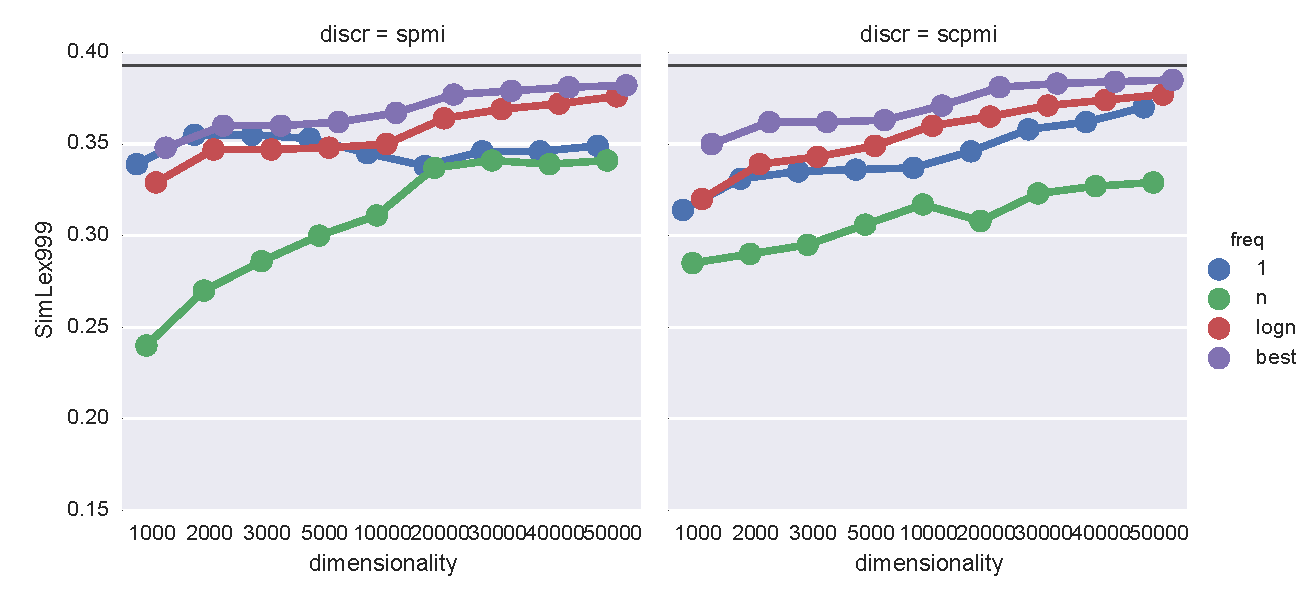
\includegraphics[width=\textwidth]{supplement/figures/SimLex999-best}
    \caption{\scriptsize \textbf{SimLex-999.}
      PPMI: 0.393.
      SVD: 0.432,
      SGNS: 0.438,
      GloVe: 0.398.
      This work: 0.385,
    }
    \label{fig:best-simlex}
  \end{subfigure}
  ~
  \begin{subfigure}[t]{0.37\textwidth}
    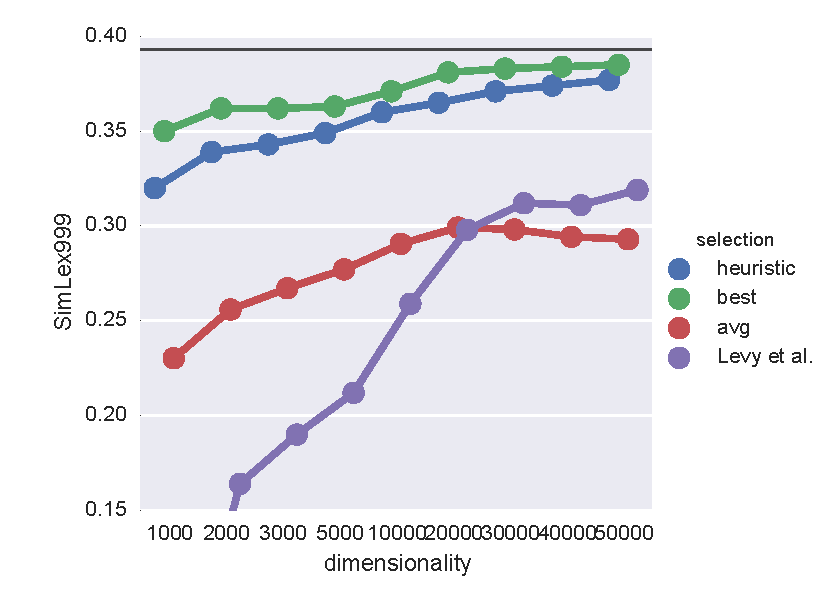
\includegraphics[width=\textwidth]{supplement/figures/SimLex999-global-best}
    \caption{}
    \label{fig:global-best-simlex}
  \end{subfigure}

  \begin{subfigure}[t]{0.6\textwidth}
    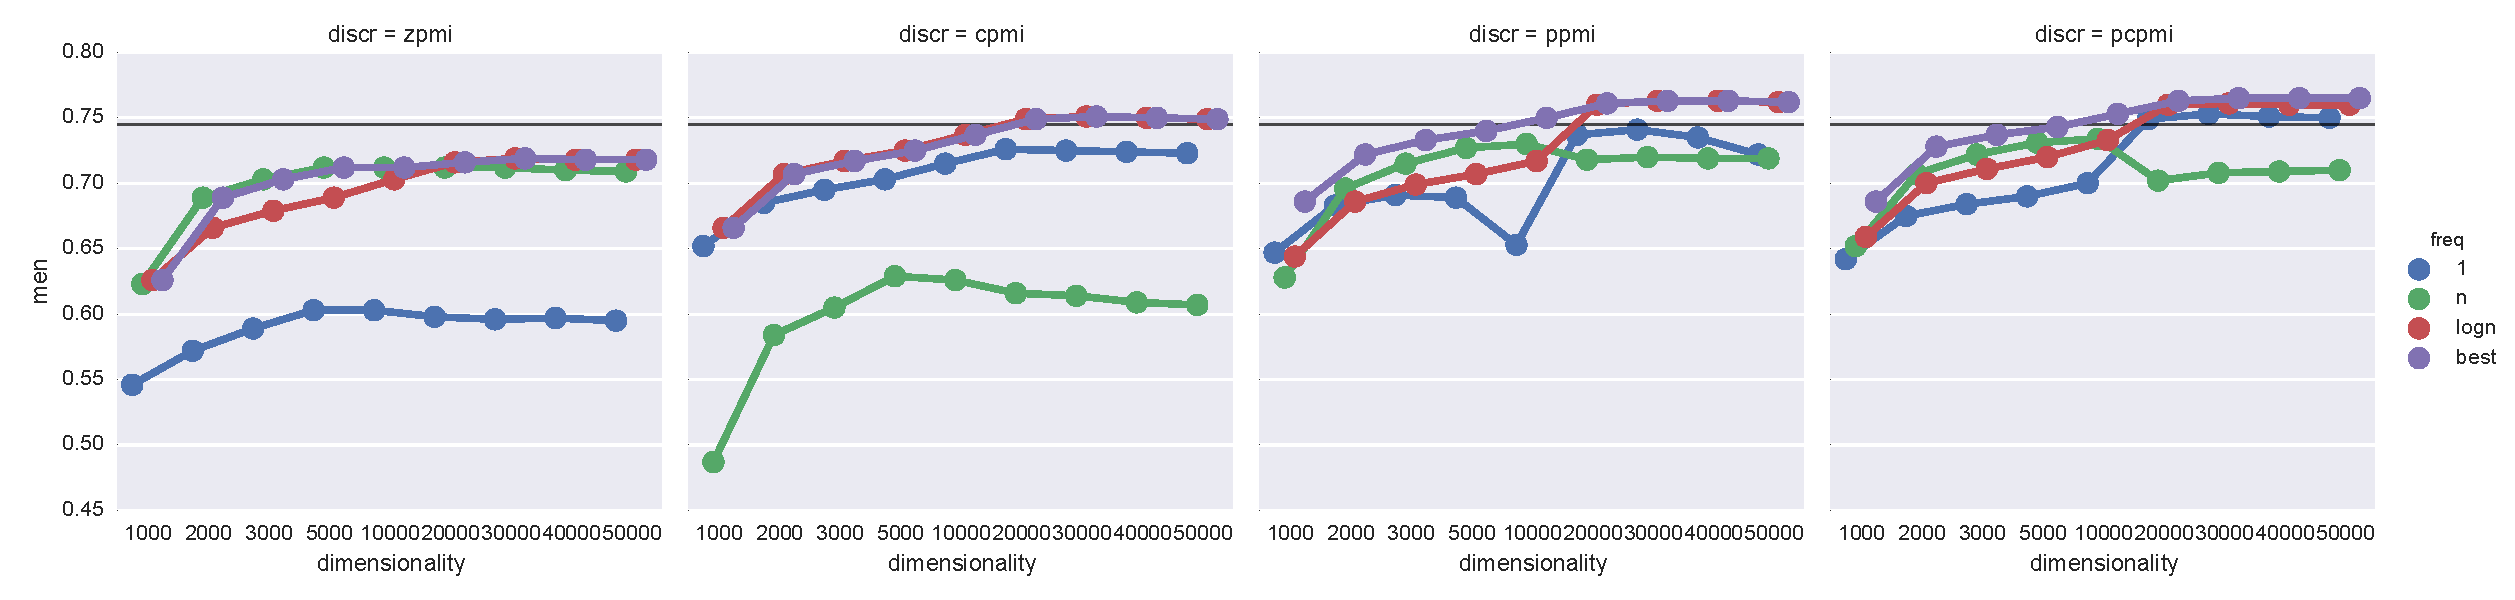
\includegraphics[width=\textwidth]{supplement/figures/men-best}
    \caption{\scriptsize \textbf{MEN.}
      PPMI: 0.745.
      SVD: 0.778,
      SGNS: 0.774,
      GloVe: 0.729.
      This work: 0.765,
    }
    \label{fig:best-men}
  \end{subfigure}
  ~
  \begin{subfigure}[t]{0.37\textwidth}
    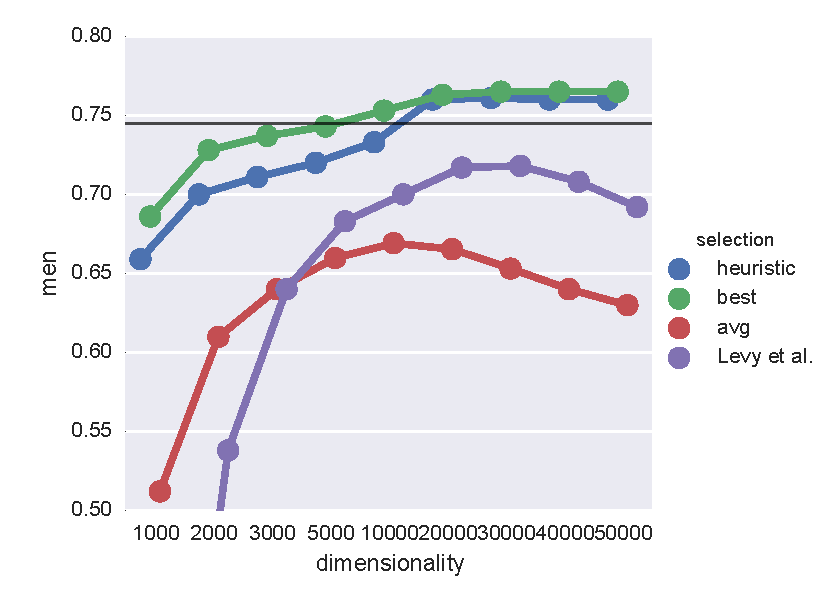
\includegraphics[width=\textwidth]{supplement/figures/men-global-best}
    \caption{}
    \label{fig:global-best-men}
  \end{subfigure}

  \caption{\small\textbf{Best configurations.} The black lines show the best count models (PPMI) reported by \protect\newcite{TACL570}. We also give our best score, SVD, SGNS and GloVe numbers from that study for comparison. On the right, our heuristic in comparison to the best and average results together with the models selected using the recommendations presented in \protect\newcite{TACL570}.}
  \label{fig:best}
\end{figure*}

%%% Local Variables:
%%% mode: latex
%%% TeX-master: "paper"
%%% End:
